% !TeX program = xelatex
\documentclass[a4paper,10pt]{article}

% ============================================================================
% កញ្ចប់បណ្ណាល័យ (Packages) – តាមលំនាំស្តង់ដារ អនុវិទ្យាល័យព្រះក្រសាំង (ls_plan.tex)
% បរិបទ៖ ថ្នាក់រៀនគ្មានស្លាយ LCD – បង្រៀនដោយប្រើក្ដារខៀន និងសន្លឹកកិច្ចការសិស្សស-ខ្មៅជាគោល
% ============================================================================
\usepackage[a4paper, left=0.95cm, right=0.95cm, top=0.85cm, bottom=0.92cm, footskip=0.52cm]{geometry}
\usepackage{amsmath}
\usepackage{unicode-math}
\usepackage{fontspec}
\usepackage{array, longtable, multirow, colortbl}
\usepackage[table]{xcolor}
\usepackage{enumitem}
\usepackage{pifont}
\usepackage{fancyhdr}
\usepackage{tikz}
\usetikzlibrary{calc, arrows.meta, angles, quotes, decorations.markings, positioning, babel}

\makeatletter
\let\@expl@@@mark@update@singlecol@structures@@\relax
\makeatother

% ============================================================================
% ការកំណត់ពុម្ពអក្សរផ្លូវការ (Cross-Platform Fonts Configuration)
% ============================================================================
\providecommand{\NGSFindFonts}{%
  \IfFileExists{C:/Windows/Fonts/cambria.ttc}{%
    \def\NGSSysPath{C:/Windows/Fonts/}%
    \def\NGSUserPath{C:/Users/KIT/AppData/Local/Microsoft/Windows/Fonts/}%
  }{%
    \IfFileExists{./fonts/KhmerOSsiemreap.ttf}{\def\NGSSysPath{./fonts/}\def\NGSUserPath{./fonts/}}{%
    \IfFileExists{../fonts/KhmerOSsiemreap.ttf}{\def\NGSSysPath{../fonts/}\def\NGSUserPath{../fonts/}}{%
    \IfFileExists{../../fonts/KhmerOSsiemreap.ttf}{\def\NGSSysPath{../../fonts/}\def\NGSUserPath{../../fonts/}}{%
    \IfFileExists{../../../fonts/KhmerOSsiemreap.ttf}{\def\NGSSysPath{../../../fonts/}\def\NGSUserPath{../../../fonts/}}{%
    \IfFileExists{../../../../fonts/KhmerOSsiemreap.ttf}{\def\NGSSysPath{../../../../fonts/}\def\NGSUserPath{../../../../fonts/}}{%
    \IfFileExists{../../../../../fonts/KhmerOSsiemreap.ttf}{\def\NGSSysPath{../../../../../fonts/}\def\NGSUserPath{../../../../../fonts/}}{%
    \IfFileExists{../../../../../../fonts/KhmerOSsiemreap.ttf}{\def\NGSSysPath{../../../../../../fonts/}\def\NGSUserPath{../../../../../../fonts/}}{%
      \def\NGSSysPath{../../../../../../../fonts/}\def\NGSUserPath{../../../../../../../fonts/}%
    }}}}}}}%
  }%
}
\NGSFindFonts

\setmathfont[Path={\NGSSysPath}, FontIndex=1, Scale=1.02]{cambria.ttc}
\defaultfontfeatures{Ligatures=TeX}

\setmainfont[
  Path={\NGSUserPath},
  Extension=.ttf,
  Script=Khmer,
  BoldFont={KhmerOSsiemreap},
  BoldFeatures={FakeBold=1.8},
  ItalicFont={KhmerOSsiemreap},
  ItalicFeatures={FakeSlant=0.25},
  BoldItalicFont={KhmerOSsiemreap},
  BoldItalicFeatures={FakeBold=1.8, FakeSlant=0.25}
]{KhmerOSsiemreap}

\newfontfamily\muol[Path={\NGSUserPath}, Extension=.ttf, Script=Khmer]{KhmerOSmuollight}
\newfontfamily\TimesEn[Path={\NGSSysPath}, Extension=.ttf, BoldFont={timesbd}, ItalicFont={timesi}, BoldItalicFont={timesbi}]{times}
\newfontfamily\NagaBold[Path={\NGSUserPath}, Extension=.ttf]{AKbalthom Naga Bold}
\newfontfamily\CalibriFont[Path={\NGSSysPath}, Extension=.ttf]{calibri}
\newfontfamily\Tacteing[Path={\NGSUserPath}]{TACTENG.TTF}
\newfontfamily\CourierBullet[Path={\NGSSysPath}, Extension=.ttf]{cour}
\newcommand{\wcirc}{{\CourierBullet\fontsize{9.5pt}{11pt}\selectfont o}}

\XeTeXlinebreaklocale "km"
\XeTeXlinebreakskip = 0pt plus 1pt minus 0.1pt

\definecolor{stepgray}{HTML}{D9D9D9}
\definecolor{headgray}{HTML}{F2F2F2}
\definecolor{boxgray}{HTML}{D9D9D9}
\definecolor{darkred}{HTML}{C00000}
\definecolor{red5e}{HTML}{FF0000}

\pagestyle{fancy}
\fancyhf{}
\renewcommand{\headrulewidth}{0pt}
\fancyfoot[R]{\CalibriFont\fontsize{11pt}{13pt}\selectfont\thepage}

\setlength{\parindent}{0pt}
\setlength{\parskip}{0pt}
\setlength{\tabcolsep}{3.8pt}

\newcolumntype{L}[1]{>{\raggedright\arraybackslash}p{#1}}

\newcommand{\en}[1]{{\TimesEn #1}}
\newcommand{\enbf}[1]{{\TimesEn\textbf{#1}}}
\newcommand{\unit}[1]{\,\text{\en{#1}}}
\newcommand{\fiveE}[1]{{\NagaBold\fontsize{9.5pt}{13pt}\selectfont\textcolor{red5e}{#1}}}
\newcommand{\timenote}[1]{\textcolor{darkred}{\textit{#1}}}
\newcommand{\redsub}[1]{\textcolor{darkred}{#1}}
\newcommand{\graybox}[1]{\colorbox{boxgray}{\strut\hspace{2pt}#1\hspace{2pt}}}
\newcommand{\ditem}{\tikz[baseline=-0.5ex]\fill (0,0.42ex) -- (0.42ex,0) -- (0,-0.42ex) -- (-0.42ex,0) -- cycle;\hspace{0.3em}}
\newcommand{\cnum}[1]{{\fontsize{10.5pt}{12pt}\selectfont\ding{\numexpr171+#1\relax}}\hspace{0.2em}}
\newcommand{\cfig}[1]{\par\vspace{4pt}{\centering #1\par}\vspace{4pt}}
\newcommand{\stepheader}[1]{\multicolumn{3}{|c|}{\cellcolor{stepgray}\muol #1} \\* \noalign{\hrule height 0.4pt}}
\newcommand{\tri}[1]{\ensuremath{\triangle #1}}
\newcommand{\ang}[1]{\ensuremath{\angle #1}}
\newcommand{\cg}{\ensuremath{\cong}}
\newcommand{\khmflourish}{{\Tacteing\fontsize{36pt}{14pt}\selectfont\raisebox{-5pt}{3}}}

\tikzset{
  tk1/.style={postaction={decorate},decoration={markings,mark=at position 0.50 with {\draw[black, line width=0.85pt](0,-0.095)--(0,0.095);}}},
  tk2/.style={postaction={decorate},decoration={markings,
    mark=at position 0.45 with {\draw[black, line width=0.85pt](0,-0.095)--(0,0.095);},
    mark=at position 0.55 with {\draw[black, line width=0.85pt](0,-0.095)--(0,0.095);}}},
  tk3/.style={postaction={decorate},decoration={markings,
    mark=at position 0.42 with {\draw[black, line width=0.85pt](0,-0.095)--(0,0.095);},
    mark=at position 0.50 with {\draw[black, line width=0.85pt](0,-0.095)--(0,0.095);},
    mark=at position 0.58 with {\draw[black, line width=0.85pt](0,-0.095)--(0,0.095);}}}
}

% ============================================================================
% ម៉ាក្រូរូបភាពធរណីមាត្រស-ខ្មៅ (Proportional 4.2–7.2 cm B&W TikZ Diagrams)
% ============================================================================

% ១. រំលឹកមេរៀនទាក់ទង៖ ចតុកោណកែង ធៀបនឹង ត្រីកោណសមបាតមានមេដ្យាន AO \perp BD
\newcommand{\figPrereqRHOM}{%
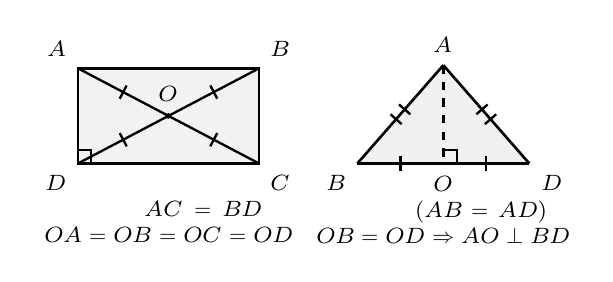
\begin{tikzpicture}[scale=0.78, every node/.style={font=\footnotesize, text=black}]
  % ឆ្វេង៖ ចតុកោណកែង (AC=BD, មិនកែងគ្នាជាទូទៅ)
  \begin{scope}[shift={(0,0)}]
    \coordinate (D) at (0,0); \coordinate (C) at (2.95,0);
    \coordinate (A) at (0,1.55); \coordinate (B) at (2.95,1.55);
    \coordinate (O) at (1.475,0.775);
    \fill[gray!10] (A)--(B)--(C)--(D)--cycle;
    \draw[black, line width=0.95pt] (A)--(B)--(C)--(D)--cycle;
    \draw[black, line width=0.85pt, tk1] (A)--(O); \draw[black, line width=0.85pt, tk1] (O)--(C);
    \draw[black, line width=0.85pt, tk1] (B)--(O); \draw[black, line width=0.85pt, tk1] (O)--(D);
    \draw[black, line width=0.7pt] (0,0.22)--(0.22,0.22)--(0.22,0);
    \fill[black] (O) circle (1.3pt) node[above=1.5pt] {$O$};
    \node[above left=1pt] at (A) {$A$}; \node[above right=1pt] at (B) {$B$};
    \node[below right=1pt] at (C) {$C$}; \node[below left=1pt] at (D) {$D$};
    \node[anchor=north, text width=3.35cm, align=center] at (1.48,-0.45) {ចតុកោណកែង៖ $AC=BD$\\$OA=OB=OC=OD$};
  \end{scope}
  % ស្ដាំ៖ ត្រីកោណសមបាត ABD (AB=AD, OB=OD => AO \perp BD)
  \begin{scope}[shift={(4.55,0)}]
    \coordinate (B) at (0,0); \coordinate (D) at (2.80,0);
    \coordinate (O) at (1.40,0); \coordinate (A) at (1.40,1.60);
    \fill[gray!12] (A)--(B)--(D)--cycle;
    \draw[black, line width=0.95pt, tk2] (A)--(B);
    \draw[black, line width=0.95pt, tk2] (A)--(D);
    \draw[black, line width=0.95pt, tk1] (B)--(O);
    \draw[black, line width=0.95pt, tk1] (O)--(D);
    \draw[black, line width=0.9pt, dashed] (A)--(O);
    \draw[black, line width=0.7pt] (1.40,0.22)--(1.62,0.22)--(1.62,0);
    \node[above=1pt] at (A) {$A$}; \node[below left=1pt] at (B) {$B$};
    \node[below=1pt] at (O) {$O$}; \node[below right=1pt] at (D) {$D$};
    \node[anchor=north, text width=3.35cm, align=center] at (1.40,-0.45) {ត្រីកោណសមបាត ($AB=AD$)៖\\$OB=OD \Rightarrow AO\perp BD$};
  \end{scope}
\end{tikzpicture}}

% ២. E1 Engage: ក្រឡាផាមួងចតុកោណស្មើ ABCD ទល់នឹង គ្រោងឫស្សីខ្លែងខ្មែរ EFGH
\newcommand{\figEngageRHOM}{%
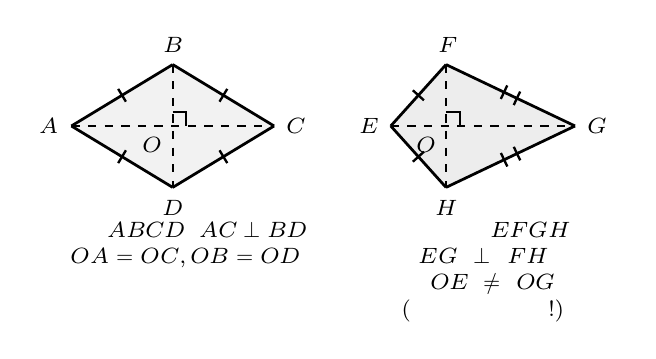
\begin{tikzpicture}[scale=0.78, every node/.style={font=\footnotesize, text=black}]
  % ឆ្វេង៖ ចតុកោណស្មើ ABCD (OA=OC, OB=OD, AC \perp BD)
  \begin{scope}[shift={(0,0.85)}]
    \coordinate (A) at (-1.65,0); \coordinate (C) at (1.65,0);
    \coordinate (B) at (0,1.00); \coordinate (D) at (0,-1.00);
    \coordinate (O) at (0,0);
    \fill[gray!10] (A)--(B)--(C)--(D)--cycle;
    \draw[black, line width=1.0pt, tk1] (A)--(B); \draw[black, line width=1.0pt, tk1] (B)--(C);
    \draw[black, line width=1.0pt, tk1] (C)--(D); \draw[black, line width=1.0pt, tk1] (D)--(A);
    \draw[black, line width=0.85pt, dashed] (A)--(C) (B)--(D);
    \draw[black, line width=0.7pt] (0,0.22)--(0.22,0.22)--(0.22,0);
    \node[left=1pt] at (A) {$A$}; \node[above=1pt] at (B) {$B$};
    \node[right=1pt] at (C) {$C$}; \node[below=1pt] at (D) {$D$};
    \node[below left=0.5pt] at (O) {$O$};
    \node[anchor=north, text width=3.45cm, align=center] at (0,-1.40) {ក្រឡាផាមួង $ABCD$៖ $AC\perp BD$\\និង $OA=OC, OB=OD$};
  \end{scope}
  % ស្ដាំ៖ គ្រោងខ្លែងខ្មែរ EFGH (EG \perp FH, OF=OH តែ OE \neq OG!)
  \begin{scope}[shift={(4.45,0.85)}]
    \coordinate (E) at (-0.90,0); \coordinate (G) at (2.10,0);
    \coordinate (F) at (0,1.00); \coordinate (H) at (0,-1.00);
    \coordinate (O) at (0,0);
    \fill[gray!14] (E)--(F)--(G)--(H)--cycle;
    \draw[black, line width=1.0pt, tk1] (E)--(F); \draw[black, line width=1.0pt, tk1] (H)--(E);
    \draw[black, line width=1.0pt, tk2] (F)--(G); \draw[black, line width=1.0pt, tk2] (G)--(H);
    \draw[black, line width=0.85pt, dashed] (E)--(G) (F)--(H);
    \draw[black, line width=0.7pt] (0,0.22)--(0.22,0.22)--(0.22,0);
    \node[left=1pt] at (E) {$E$}; \node[above=1pt] at (F) {$F$};
    \node[right=1pt] at (G) {$G$}; \node[below=1pt] at (H) {$H$};
    \node[below left=0.5pt] at (O) {$O$};
    \node[anchor=north, text width=3.45cm, align=center] at (0.60,-1.40) {គ្រោងខ្លែងខ្មែរ $EFGH$៖ $EG\perp FH$\\តែ $OE\neq OG$ (ជ្រុងមិនស្មើគ្នាទាំង ៤!)};
  \end{scope}
\end{tikzpicture}}

% ៣. E3 Explain: លក្ខណៈចតុកោណស្មើ (ទ្រឹស្ដីបទទី១-៤៖ អង្កត់ទ្រូងកែង និងពុះមុំឈម)
\newcommand{\figTheoremsRHOM}{%
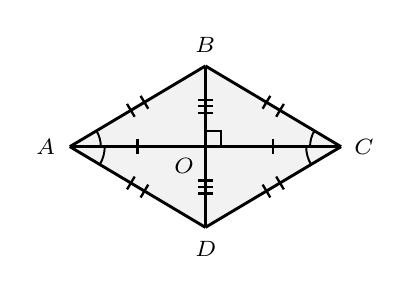
\begin{tikzpicture}[scale=0.82, every node/.style={font=\footnotesize, text=black}]
  \coordinate (A) at (-2.10,0); \coordinate (C) at (2.10,0);
  \coordinate (B) at (0,1.25); \coordinate (D) at (0,-1.25);
  \coordinate (O) at (0,0);
  \fill[gray!10] (A)--(B)--(C)--(D)--cycle;
  \draw[black, line width=1.05pt, tk2] (A)--(B);
  \draw[black, line width=1.05pt, tk2] (B)--(C);
  \draw[black, line width=1.05pt, tk2] (C)--(D);
  \draw[black, line width=1.05pt, tk2] (D)--(A);
  \draw[black, line width=0.95pt, tk1] (A)--(O); \draw[black, line width=0.95pt, tk1] (O)--(C);
  \draw[black, line width=0.95pt, tk3] (B)--(O); \draw[black, line width=0.95pt, tk3] (O)--(D);
  \draw[black, line width=0.75pt] (0,0.24)--(0.24,0.24)--(0.24,0);
  % ធ្នូមុំពុះត្រង់ A និង C
  \draw[black, line width=0.7pt] ($(A)+(30.8:0.48)$) arc (30.8:0:0.48);
  \draw[black, line width=0.7pt] ($(A)+(0:0.54)$) arc (0:-30.8:0.54);
  \draw[black, line width=0.7pt] ($(C)+(180:0.48)$) arc (180:149.2:0.48);
  \draw[black, line width=0.7pt] ($(C)+(210.8:0.54)$) arc (210.8:180:0.54);
  \node[left=1.5pt] at (A) {$A$}; \node[above=1.5pt] at (B) {$B$};
  \node[right=1.5pt] at (C) {$C$}; \node[below=1.5pt] at (D) {$D$};
  \node[below left=1pt] at (O) {$O$};
\end{tikzpicture}}

% ៤. E4 Elaborate: គំរូទី១ (ទំ.១៧៨-១៧៩៖ AOBI ចតុកោណស្មើ) & គំរូទី២ (លំ.១២ ទំ.១៨៦៖ AD=CE)
\newcommand{\figModelRHOM}{%
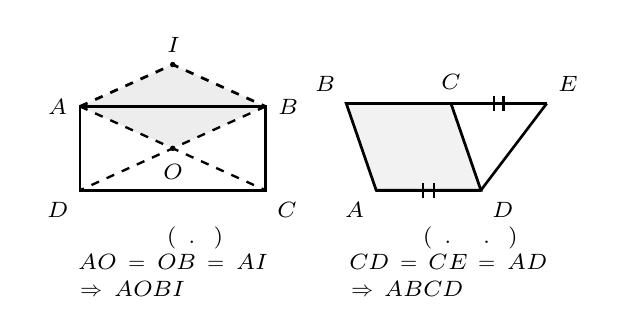
\begin{tikzpicture}[scale=0.76, every node/.style={font=\footnotesize, text=black}]
  % ឆ្វេង៖ លំហាត់គំរូ ទំ.១៧៨-១៧៩ (ចតុកោណកែង ABCD ផ្ចិត O, ប្រលេឡូក្រាម AOBI)
  \begin{scope}[shift={(0,0)}]
    \coordinate (D) at (0,0); \coordinate (C) at (3.10,0);
    \coordinate (A) at (0,1.40); \coordinate (B) at (3.10,1.40);
    \coordinate (O) at (1.55,0.70); \coordinate (I) at (1.55,2.10);
    \fill[gray!14] (A)--(I)--(B)--(O)--cycle;
    \draw[black, line width=0.95pt] (A)--(B)--(C)--(D)--cycle;
    \draw[black, line width=0.85pt, dashed] (A)--(C) (B)--(D);
    \draw[black, line width=1.0pt, dashed] (A)--(I)--(B);
    \fill[black] (O) circle (1.3pt) node[below=2pt] {$O$};
    \fill[black] (I) circle (1.3pt) node[above=1pt] {$I$};
    \node[left=1pt] at (A) {$A$}; \node[right=1pt] at (B) {$B$};
    \node[below right=1pt] at (C) {$C$}; \node[below left=1pt] at (D) {$D$};
    \node[anchor=north, text width=3.45cm, align=center] at (1.55,-0.45) {គំរូទី១ (ទំ.១៧៩)៖ $AO=OB=AI$\\$\Rightarrow AOBI$ ជាចតុកោណស្មើ};
  \end{scope}
  % ស្ដាំ៖ លំហាត់ទី១២ ទំ.១៨៦ (ប្រលេឡូក្រាម ABCD, E លើបន្លាយ BC, AD=CE, \angle CDE=\angle CED)
  \begin{scope}[shift={(4.45,0)}]
    \coordinate (B) at (0,1.45); \coordinate (C) at (1.75,1.45); \coordinate (E) at (3.35,1.45);
    \coordinate (A) at (0.50,0); \coordinate (D) at (2.25,0);
    \fill[gray!10] (A)--(B)--(C)--(D)--cycle;
    \draw[black, line width=1.0pt] (A)--(B)--(C)--(D)--cycle;
    \draw[black, line width=0.95pt, tk2] (A)--(D);
    \draw[black, line width=0.95pt, tk2] (C)--(E);
    \draw[black, line width=0.95pt] (D)--(E);
    \node[below left=1pt] at (A) {$A$}; \node[above left=1pt] at (B) {$B$};
    \node[above=1.5pt] at (C) {$C$}; \node[below right=1pt] at (D) {$D$};
    \node[above right=1pt] at (E) {$E$};
    \node[anchor=north, text width=3.45cm, align=center] at (1.70,-0.45) {គំរូទី២ (លំ.១២ ទំ.១៨៦)៖ $CD=CE=AD$\\$\Rightarrow ABCD$ ជាចតុកោណស្មើ};
  \end{scope}
\end{tikzpicture}}

% ៥. E5 Evaluate: ប្រតិបត្តិ ទំ.១៧៩ (ចតុកោណស្មើ ABCD ដែលមាន AB=BC=CD=DA=BD)
\newcommand{\figPractRHOM}{%
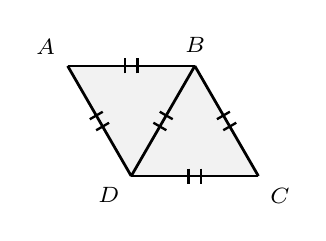
\begin{tikzpicture}[scale=0.85, every node/.style={font=\footnotesize, text=black}]
  \coordinate (D) at (0.95,0); \coordinate (C) at (2.85,0);
  \coordinate (A) at (0,1.645); \coordinate (B) at (1.90,1.645);
  \fill[gray!10] (A)--(B)--(C)--(D)--cycle;
  \draw[black, line width=1.0pt, tk2] (A)--(B);
  \draw[black, line width=1.0pt, tk2] (B)--(C);
  \draw[black, line width=1.0pt, tk2] (C)--(D);
  \draw[black, line width=1.0pt, tk2] (D)--(A);
  \draw[black, line width=1.0pt, tk2] (B)--(D);
  \node[above left=1pt] at (A) {$A$}; \node[above=1.5pt] at (B) {$B$};
  \node[below right=1pt] at (C) {$C$}; \node[below left=1pt] at (D) {$D$};
\end{tikzpicture}}

\begin{document}
\fontsize{10pt}{15.2pt}\selectfont

% -------------------- ក្បាលកិច្ចតែងការ (Header) --------------------
\begin{center}
  {\muol\fontsize{11pt}{16pt}\selectfont ព្រះរាជាណាចក្រកម្ពុជា}\\[2pt]
  {\muol\fontsize{10pt}{15pt}\selectfont ជាតិ សាសនា ព្រះមហាក្សត្រ}\\[1pt]
  \khmflourish
\end{center}

\vspace{-28pt}
{\muol\fontsize{9.5pt}{12.5pt}\selectfont
មន្ទីរអប់រំ យុវជន និងកីឡា ខេត្តកំពង់ធំ\\
ការិយាល័យអប់រំ យុវជន និងកីឡា ស្រុកកំពង់ស្វាយ\\
អនុវិទ្យាល័យព្រះក្រសាំង}

\vspace{1pt}
\begin{center}
  {\muol\fontsize{10pt}{14pt}\selectfont កិច្ចតែងការបង្រៀន}
\end{center}
\vspace{0pt}

% -------------------- ព័ត៌មានទូទៅ (Metadata) --------------------
{\renewcommand{\arraystretch}{0.95}
\hspace*{4.05cm}%
\begin{tabular}{@{}l l l@{}}
  - \hspace{0.35cm} មុខវិជ្ជា & : & គណិតវិទ្យា ថ្នាក់ទី៨ \\
  - \hspace{0.35cm} ចំណងជើងមេរៀន & : & មេរៀនទី១៣ ចតុកោណ \\
  - \hspace{0.35cm} ចំណងជើងរង & : & ២.៣ លក្ខណៈចតុកោណស្មើ (ទំ.១៧៦--១៧៩ និងទំ.១៨៥--១៨៦) \\
  - \hspace{0.35cm} រយៈពេល & : & ១ ម៉ោងសិក្សា (៥០ នាទី) \\
  - \hspace{0.35cm} បង្រៀនដោយ & : & ហុក ប៊ុនថែន \\
  - \hspace{0.35cm} កាលបរិច្ឆេទ & : & ថ្ងៃពុធ ៧កើត ខែមិគសិរ ព.ស.២៥៧០ (១៦ ធ្នូ ២០២៦) \\
\end{tabular}

\vspace{1pt}

% -------------------- I. វត្ថុបំណង --------------------
\textbf{I.} {\muol វត្ថុបំណង}\\[1pt]
\hspace*{0.55cm}%
\begin{tabular}{@{}l l L{14.2cm}@{}}
  \wcirc \hspace{0.25cm} វិជ្ជាសម្បទា & : & សិស្សពោលបានត្រឹមត្រូវនូវនិយមន័យចតុកោណស្មើ (ប្រលេឡូក្រាមមានជ្រុងជាប់ពីរប៉ុនគ្នា) ទ្រឹស្ដីបទទី១ (ជ្រុងទាំងបួនប៉ុនគ្នា) ទ្រឹស្ដីបទទី២ (អង្កត់ទ្រូងកែងគ្នា) ទ្រឹស្ដីបទទី៣ (ប្រលេឡូក្រាមមានអង្កត់ទ្រូងកែងគ្នាជាចតុកោណស្មើ) និងទ្រឹស្ដីបទទី៤ (អង្កត់ទ្រូងជាកន្លះបន្ទាត់ពុះមុំឈម) តាមសៀវភៅគោល ទំ.១៧៦--១៧៨ ។ \\
  \wcirc \hspace{0.25cm} បំណិនសម្បទា & : & សិស្សស្រាយបញ្ជាក់ទ្រឹស្ដីបទទី២--៤ តាមត្រីកោណប៉ុនគ្នាជុំវិញផ្ចិត $O$ លើសន្លឹកកិច្ចការស-ខ្មៅ ព្រមទាំងដោះស្រាយលំហាត់សម្រាយបញ្ជាក់ និងគណនាមុំក្នុងចតុកោណស្មើដោយប្រើធនាគារហេតុផល \cnum{1}--\cnum{5} ។ \\
  \wcirc \hspace{0.25cm} ចរិយាសម្បទា & : & សិស្សមានទម្លាប់បែងចែកច្បាស់លាស់រវាងចតុកោណស្មើ និងចតុកោណខ្លែង (មិនសន្និដ្ឋានថាឱ្យតែអង្កត់ទ្រូងកែងគ្នាសុទ្ធតែជាចតុកោណស្មើដោយភ្លេចពិនិត្យចំណុចកណ្ដាលឡើយ) ព្រមទាំងឱ្យតម្លៃលើក្បាច់ក្រឡាចតុកោណស្មើនៃហូលផាមួងខ្មែរ ។ \\
\end{tabular}

\vspace{1pt}

% -------------------- II. សម្ភារៈឧបទេស --------------------
\textbf{II.} {\muol សម្ភារៈឧបទេស}\\[1pt]
\hspace*{0.55cm}$\bullet$ \hspace{0.35cm} សៀវភៅសិក្សាគោលគណិតវិទ្យាថ្នាក់ទី៨ (ទំ.១៧៦--១៧៩ និង ១៨៥--១៨៦) ក្ដារខៀន ដីស បន្ទាត់ក្រិត រ៉ាប់ព័រទ័រ ដែកឈាន និងសន្លឹកកិច្ចការសិស្សស-ខ្មៅ (\en{Worksheet\_RHOM1} ចំនួន ២ ទំព័រ \en{A4} ដោយគ្មានស្លាយ \en{LCD}) ។

\vspace{1pt}

% -------------------- III. វិធីសាស្រ្តបង្រៀន --------------------
\textbf{III.} {\muol វិធីសាស្រ្តបង្រៀន}\\[1pt]
\hspace*{0.45cm}%
\begin{tabular}{@{}l l L{14.85cm}@{}}
  $\bullet$ \hspace{0.25cm} គោលវិធី & : & សិស្សមជ្ឈមណ្ឌល (សិក្សាប្រៀបធៀបជាដៃគូលើសន្លឹកកិច្ចការបំពេញផ្ទាល់ គ្មានស្លាយ \en{LCD}) \\
  $\bullet$ \hspace{0.25cm} យុទ្ធវិធីបង្រៀន & : & គម្រូស្ថាបនានិយម \en{5Es} រួមបញ្ចូល \textbf{វិធីប្រៀបធៀបករណីផ្ទុយគ្នា — ចតុកោណស្មើ ទល់នឹង ខ្លែង និងចតុកោណកែង} (\en{Contrastive Case Comparison — Rittle-Johnson \& Star, 2007; Fujita, 2012}) \\
\end{tabular}
}

\vspace{1pt}

% -------------------- IV. ដំណើរការបង្រៀន --------------------
\textbf{IV.} {\muol ដំណើរការបង្រៀន}

\vspace{1pt}

\renewcommand{\arraystretch}{1.15}
\begin{longtable}{|L{5.50cm}|L{7.90cm}|L{4.80cm}|}
\hline
\rowcolor{headgray}
\multicolumn{1}{|c|}{\muol សកម្មភាពគ្រូ} &
\multicolumn{1}{c|}{\muol ខ្លឹមសារមេរៀន} &
\multicolumn{1}{c|}{\muol សកម្មភាពសិស្ស} \\
\hline
\endhead
\hline
\endfoot
\hline
\endlastfoot

% ==================== ជំហានទី១ (2min) ====================
\stepheader{ជំហានទី១ \enbf{(}រដ្ឋបាលថ្នាក់\enbf{)}}
$\bullet$ ពិនិត្យអវត្តមាន សណ្ដាប់ធ្នាប់ អនាម័យ និងសម្ភារៈធរណីមាត្រ (បន្ទាត់ក្រិត រ៉ាប់ព័រទ័រ ដែកឈាន)
&
$\bullet$ ពិនិត្យវត្តមាន និងសណ្ដាប់ធ្នាប់ថ្នាក់រៀន \par
$\bullet$ ត្រៀមបន្ទាត់ក្រិត រ៉ាប់ព័រទ័រ និងដែកឈាន
&
$\circ$ ប្រធានថ្នាក់រាយការណ៍អវត្តមាន និងត្រៀមឧបករណ៍ធរណីមាត្រ \\[3pt]

$\bullet$ រៀបចំសិស្សជាដៃគូពិភាក្សា រួចចែកសន្លឹកកិច្ចការ \en{Worksheet\_RHOM1} (២ ទំព័រ \en{A4}) ផ្កាប់លើតុ
&
$\bullet$ ការចាត់ដៃគូសិក្សា និងចែកសន្លឹកកិច្ចការស-ខ្មៅ
&
$\circ$ អង្គុយតាមដៃគូ និងទទួលសន្លឹកកិច្ចការទុកលើតុ \\
\hline

% ==================== ជំហានទី២ (9min: <=3 + 3 + E1 3) ====================
\stepheader{ជំហានទី២ \enbf{(}កិច្ចការផ្ទះ \enbf{+} ទំនាក់ទំនងមេរៀនថ្មី\enbf{)}}
\ditem \textbf{កំណែកិច្ចការផ្ទះ ($\le 3\unit{min}$)} \timenote{សង្ខេបខ្លីលើក្ដារខៀន}
&
{\centering\redsub{កំណែកិច្ចការផ្ទះ (ម៉ោងមុន៖ លក្ខណៈចតុកោណកែង)}\par}
&
$\circ$ យកសៀវភៅកិច្ចការផ្ទះមកផ្ទៀងផ្ទាត់ \\[2pt]

$\bullet$ ផ្ទៀងផ្ទាត់ចម្លើយលំហាត់ទី១ និងលំហាត់ទី២ យ៉ាងរហ័សលើក្ដារខៀន
&
$\bullet$ \textbf{លំ.១៖} $BF=5\unit{cm}\Rightarrow BE=10\unit{cm}$ ។ នោះ $AC=BE=CD=10\unit{cm} \Rightarrow \tri{ACD}$ ជាត្រីកោណសមបាតកំពូល $C$ ។ \par
$\bullet$ \textbf{លំ.២៖} $2x+1=7\Rightarrow x=3 \Rightarrow AC=14\unit{cm}=BD \Rightarrow ABCD$ ជាចតុកោណកែង ។
&
$\circ$ ផ្ទៀងផ្ទាត់ចម្លើយ និងកែលម្អចំណុចខ្វះខាត \\[3pt]

\ditem \textbf{រំលឹកមេរៀនទាក់ទង ($3\unit{min}$)} \par
$\bullet$ គូសរូបលើក្ដារខៀន សួររំលឹក៖ ១. តើអង្កត់ទ្រូងចតុកោណកែងកែងគ្នាជាទូទៅឬទេ? ២. ក្នុងត្រីកោណសមបាត $\tri{ABD}$ ($AB=AD$) បើ $O$ ជាចំណុចកណ្ដាល $BD$ តើ $AO$ និង $BD$ មានទំនាក់ទំនងអ្វី?
&
{\centering\redsub{រំលឹកមេរៀនទាក់ទងមេរៀនថ្មី}\par} \par
$\bullet$ ក្នុងចតុកោណកែងទូទៅ អង្កត់ទ្រូង $AC=BD$ តែ\textbf{មិនកែងគ្នាទេ} ។ \par
$\bullet$ ក្នុងត្រីកោណសមបាត $\tri{ABD}$ ($AB=AD$) មេដ្យាន $AO$ ក៏ជាកម្ពស់ ($AO\perp BD$) និងជាកន្លះបន្ទាត់ពុះមុំកំពូល $\ang{BAD}$ ដែរ!
&
$\circ$ ឆ្លើយផ្ទាល់មាត់៖ «អង្កត់ទ្រូងចតុកោណកែងមិនកែងគ្នាទេ តែមេដ្យានត្រីកោណសមបាតកែងនឹងបាត!» \\[3pt]

&
\cfig{\figPrereqRHOM}
& \\[3pt]

\fiveE{E1 - Engage (3min)} \timenote{(កុំទាន់ផ្ដល់ចម្លើយ)} \par
\ditem \textbf{បញ្ហាភ្ញាក់ផ្អើល «ក្បាច់ក្រឡាផាមួង ទល់នឹង គ្រោងឫស្សីខ្លែងខ្មែរ»៖} \par
$\bullet$ គូសរូបប្រៀបធៀបក្រឡាផាមួង $ABCD$ និងគ្រោងខ្លែងខ្មែរ $EFGH$ ដែលសុទ្ធតែមានអង្កត់ទ្រូងកែងគ្នាទាំងពីរ!
&
{\centering\redsub{ស្ថានភាពបញ្ហា៖ ក្រឡាផាមួង ទល់នឹង គ្រោងខ្លែងខ្មែរ}\par}
&
$\circ$ សង្កេតរូបប្រៀបធៀបលើក្ដារខៀន និងលើសន្លឹកកិច្ចការផ្នែកទី១ \\[3pt]

&
\cfig{\figEngageRHOM}
& \\[3pt]

– \textbf{សំណួរបំផុស៖} «សិស្ស ក និយាយថា៖ ឱ្យតែចតុកោណមានអង្កត់ទ្រូងកែងគ្នា ($AC\perp BD$ និង $EG\perp FH$) នោះជ្រុងទាំង ៤ របស់វាច្បាស់ជាប៉ុនគ្នាជាចតុកោណស្មើទាំងអស់! តើសិស្ស ក ត្រូវឬខុស? ហេតុអ្វីខ្លែងខ្មែរមានជ្រុងមិនស្មើគ្នាទាំង ៤?»
&
\textbf{ចម្ងល់គោលប្រចាំម៉ោង៖} \par
(១) តើចតុកោណស្មើមានលក្ខណៈជ្រុង និងអង្កត់ទ្រូងពិសេសអ្វីខ្លះ? \par
(២) តើត្រូវមានលក្ខខណ្ឌអ្វីបន្ថែមលើ $AC\perp BD$ ទើបចតុកោណមួយក្លាយជាចតុកោណស្មើពិតប្រាកដ?
&
$\circ$ ពិភាក្សាជាដៃគូ ៣០ វិនាទី រួចគូសធីកការទស្សន៍ទាយដំបូងក្នុងប្រអប់ \en{E1} លើសន្លឹកកិច្ចការ \\
\hline

% ==================== ជំហានទី៣ (17min: E2 11m + E3 6m) ====================
\stepheader{ជំហានទី៣ \enbf{(}ខ្លឹមសារមេរៀនថ្មី\enbf{)}}
\fiveE{E2 - Explore (11min)} \par
$\bullet$ សរសេរចំណងជើងរងលើក្ដារខៀន និងឱ្យសិស្សបើកសន្លឹកកិច្ចការទំព័រទី១ ផ្នែកទី២
&
២.៣ លក្ខណៈចតុកោណស្មើ (ទំ.១៧៦--១៧៩)
&
$\circ$ កត់ចំណងជើងរងចូលសៀវភៅសរសេរ និងបើកសន្លឹកកិច្ចការទំព័រទី១ \\[3pt]

\ditem \textbf{សកម្មភាពទី១៖ វាស់ប្រៀបធៀបខ្នាតពិត 1:1 លើសន្លឹកកិច្ចការ ($5\unit{min}$)} \par
$\bullet$ ឱ្យដៃគូសិស្សវាស់ចតុកោណស្មើខ្នាតពិត $ABCD$ ($OA=OC=2.4\unit{cm}, OB=OD=1.8\unit{cm}$)៖ វាស់ជ្រុងទាំង ៤, អង្កត់ទ្រូង $AC, BD$, មុំត្រង់ផ្ចិត $\ang{AOB}$ និងមុំពុះ $\ang{BAO}, \ang{DAO}$!
&
{\centering\textbf{លទ្ធផលពិសោធន៍វាស់ប្រៀបធៀប}\par} \par
$\bullet$ ជ្រុងទាំងបួនស្មើគ្នា៖ $AB=BC=CD=DA=3.0\unit{cm}$ តែអង្កត់ទ្រូង $AC=4.8\unit{cm}\neq BD=3.6\unit{cm}$ (\graybox{អង្កត់ទ្រូងចតុកោណស្មើទូទៅមិនប៉ុនគ្នាទេ!}) \par
$\bullet$ អង្កត់ទ្រូងកែងគ្នា ($\ang{AOB}=90^\circ$) និងពុះមុំ ($\ang{BAO}=\ang{DAO}\approx 37^\circ$)!
&
$\circ$ វាស់ប្រវែងជ្រុង អង្កត់ទ្រូង និងមុំជាក់ស្ដែង រួចប្រៀបធៀបជាមួយរូបខ្លែង $EFGH$ \\[3pt]

\ditem \textbf{សកម្មភាពទី២៖ សម្រាយបញ្ជាក់តាមត្រីកោណជុំវិញផ្ចិត $O$ ($6\unit{min}$)} \par
$\bullet$ ដឹកនាំសិស្សគូស \textbf{[tracing]} លើជ្រុងរួម $AO$ ក្នុង $\tri{ABO}$ និង $\tri{ADO}$ ដើម្បីបំពេញសម្រាយបញ្ជាក់ \textbf{ផ្នែក ក (ទ្រឹស្ដីបទទី២ និងទី៤)}
&
\textbf{ការស្រាយបញ្ជាក់តាមត្រីកោណប៉ុនគ្នាជុំវិញ $O$៖} \par
$\bullet$ \textbf{ផ្នែក ក (ទ្រឹស្ដីបទទី២ និងទី៤)៖} ក្នុងចតុកោណស្មើ $ABCD$ មាន $AB=AD$, $OB=OD$ និង $AO$ ជ្រុងរួម $\Rightarrow \tri{ABO}\cg\tri{ADO}$ (\textbf{ជ-ជ-ជ}) $\Rightarrow \ang{AOB}=\ang{AOD}=90^\circ$ ($AC\perp BD$) និង $\ang{BAO}=\ang{DAO}$!
&
$\circ$ គូស \textbf{[tracing]} ជ្រុងរួម $AO$ និងបំពេញសម្រាយបញ្ជាក់ \textbf{ផ្នែក ក} លើសន្លឹកកិច្ចការ \\[2pt]

$\bullet$ ណែនាំឱ្យសិស្សបំពេញ \textbf{ផ្នែក ខ (ទ្រឹស្ដីបទទី៣)}៖ ប្រលេឡូក្រាមមាន $AC\perp BD$ ជាចតុកោណស្មើ
&
$\bullet$ \textbf{ផ្នែក ខ (ទ្រឹស្ដីបទទី៣)៖} ក្នុងប្រលេឡូក្រាម $ABCD$ បើ $AC\perp BD$ នោះ $\tri{ABO}\cg\tri{ADO}$ (\textbf{ជ-ម-ជ}: $OB=OD, \ang{AOB}=\ang{AOD}=90^\circ, AO$ រួម) $\Rightarrow AB=AD \Rightarrow ABCD$ ជាចតុកោណស្មើ!
&
$\circ$ បំពេញសម្រាយបញ្ជាក់ \textbf{ផ្នែក ខ} និងរកឃើញថាលក្ខខណ្ឌ $OA=OC, OB=OD$ ជាគន្លឹះខុសពីខ្លែង \\[3pt]

\fiveE{E3 - Explain (6min)} \par
\ditem \textbf{បង្គុំនិយមន័យ ទ្រឹស្ដីបទទី១--៤ និងធនាគារហេតុផល \cnum{1}--\cnum{5}៖} \par
$\bullet$ ហៅតំណាងដៃគូឡើងបកស្រាយ រួចគ្រូសង្ខេបទ្រឹស្ដីបទផ្លូវការ (ទំ.១៧៦--១៧៨)
&
\textbf{សង្ខេបលក្ខណៈចតុកោណស្មើ និងធនាគារហេតុផល \cnum{1}--\cnum{5}៖} \par
\cnum{1} \textbf{និយមន័យ និងទ្រឹស្ដីបទទី១៖} ចតុកោណស្មើ ជាប្រលេឡូក្រាមមានជ្រុងជាប់ពីរប៉ុនគ្នា $\Rightarrow$ \textbf{ជ្រុងទាំងបួនប៉ុនគ្នា} ($AB=BC=CD=DA$) ។ \par
\cnum{2} \textbf{ទ្រឹស្ដីបទទី២៖} អង្កត់ទ្រូងនៃចតុកោណស្មើកែងគ្នា ($AC\perp BD$ ត្រង់ចំណុចកណ្ដាល $O$) ។
&
$\circ$ តំណាងដៃគូឡើងបកស្រាយ និងសិស្សបំពេញ \cnum{1}--\cnum{2} លើសន្លឹកកិច្ចការទំព័រទី២ \\[3pt]

&
\cfig{\figTheoremsRHOM}
& \\[3pt]

$\bullet$ សង្កត់ធ្ងន់លើទ្រឹស្ដីបទសម្គាល់ទី៣ ទ្រឹស្ដីបទកន្លះបន្ទាត់ពុះមុំទី៤ និងមុំបំពេញកែងក្នុងត្រីកោណកែងតូចៗ
&
\cnum{3} \textbf{ទ្រឹស្ដីបទទី៣ (សម្គាល់)៖} ប្រលេឡូក្រាមដែលមានអង្កត់ទ្រូងកែងគ្នា ជាចតុកោណស្មើ (ឬចតុកោណមានជ្រុងទាំង ៤ ប៉ុនគ្នា) ។ \par
\cnum{4} \textbf{ទ្រឹស្ដីបទទី៤៖} អង្កត់ទ្រូងនៃចតុកោណស្មើ ជាកន្លះបន្ទាត់ពុះមុំឈម និងជាអ័ក្សឆ្លុះ ។ \par
\cnum{5} \textbf{មុំបំពេញកែង៖} ក្នុង $\tri{OCD}$ កែងត្រង់ $O$ គេបាន $\ang{ODC}+\ang{OCD}=90^\circ$ ។
&
$\circ$ កត់ត្រា \cnum{3}--\cnum{5} ចូលក្នុងប្រអប់ធនាគារហេតុផល \\
\hline

% ==================== ជំហានទី៤ (20min: E4 10m + E5 10m) ====================
\stepheader{ជំហានទី៤ \enbf{(}ពង្រឹង និងពង្រីកចំណេះដឹង\enbf{)}}
\fiveE{E4 - Elaborate (10min)} \par
\ditem \textbf{លំហាត់គំរូអនុវត្តចេញពីសៀវភៅគោល (ទំ.១៧៨--១៧៩ និងលំ.១២ ទំ.១៨៦)៖} \par
$\bullet$ ដឹកនាំសិស្សវិភាគគំរូទី១ (លំហាត់គំរូ ទំ.១៧៨--១៧៩) ដោយភ្ជាប់លក្ខណៈចតុកោណកែងទៅចតុកោណស្មើ
&
{\muol លំហាត់គំរូទី១} \textbf{(លំហាត់គំរូ ទំ.១៧៨--១៧៩)៖} \par
គេមានចតុកោណកែង $ABCD$ មានអង្កត់ទ្រូងកាត់គ្នាត្រង់ $O$ ។ គេសង់ប្រលេឡូក្រាម $AOBI$ ។ បង្ហាញថា $AOBI$ ជាចតុកោណស្មើ ។
&
$\circ$ អានប្រធានគំរូទី១ និងគូសឆ្នូត \textbf{[tracing]} លើ $AO=OB$ ក្នុងចតុកោណកែង $ABCD$ \\[2pt]

$\bullet$ ដឹកនាំសិស្សវិភាគគំរូទី២ (លំហាត់ទី១២ ទំ.១៨៦) លើសន្លឹកកិច្ចការទំព័រទី២
&
{\muol លំហាត់គំរូទី២} \textbf{(លំហាត់ទី១២ ទំ.១៨៦)៖} \par
ក្នុងប្រលេឡូក្រាម $ABCD$ គេមាន $AD=CE$ និង $\ang{CDE}=\ang{CED}$ ($E$ ស្ថិតលើបន្ទាត់ $BC$) ។ បង្ហាញថា $ABCD$ ជាចតុកោណស្មើ ។
&
$\circ$ សង្កេតរូបគំរូទី២ គូសធ្នូមុំស្មើគ្នា $\ang{CDE}=\ang{CED}$ និងឆ្នូត $AD=CE$ \\[3pt]

&
\cfig{\figModelRHOM}
& \\[3pt]

$\bullet$ សួរបំផុសគំរូទី១៖ «ហេតុអ្វី $AO=OB$? ហើយតើ $AI$ ស្មើនឹងអង្កត់ណាក្នុងប្រលេឡូក្រាម $AOBI$?»
&
\textbf{ដំណោះស្រាយសង្ខេប៖} \par
$\bullet$ \textbf{គំរូទី១៖} ក្នុងចតុកោណកែង $ABCD$ គេមាន $AO=OB$ ។ ក្នុងប្រលេឡូក្រាម $AOBI$ មាន $AI=OB \Rightarrow AO=AI$ (ជ្រុងជាប់ប៉ុនគ្នា) $\Rightarrow$ \graybox{$AOBI$ ជាចតុកោណស្មើ} (តាម \cnum{1}) ។
&
$\circ$ បំពេញសម្រាយបញ្ជាក់គំរូទី១ ដោយភ្ជាប់ហេតុផល \cnum{1} \\[2pt]

$\bullet$ ដឹកនាំសម្រាយបញ្ជាក់គំរូទី២ និងសួរឆ្លុះបញ្ចាំង \en{EIA}៖ «តើមានវិធីសម្គាល់ប្រលេឡូក្រាមមួយជាចតុកោណស្មើប៉ុន្មានផ្លូវ?»
&
$\bullet$ \textbf{គំរូទី២៖} ក្នុង $\tri{CDE}$ មាន $\ang{CDE}=\ang{CED} \Rightarrow CD=CE$ (សមបាតកំពូល $C$) ។ តែ $AD=CE \Rightarrow AD=CD$ (ជ្រុងជាប់នៃប្រលេឡូក្រាម $ABCD$ ប៉ុនគ្នា) $\Rightarrow$ \graybox{$ABCD$ ជាចតុកោណស្មើ}! \par
$\bullet$ \textbf{គន្លឹះ \en{EIA}៖} ដើម្បីបញ្ជាក់ប្រលេឡូក្រាមជាចតុកោណស្មើ អាចបង្ហាញ \textbf{ជ្រុងជាប់ពីរប៉ុនគ្នា} (\cnum{1}) ឬ \textbf{អង្កត់ទ្រូងកែងគ្នា} (\cnum{3})!
&
$\circ$ បំពេញគំរូទី២ និងកត់សម្គាល់ផ្លូវសម្គាល់ទាំងពីរនៃចតុកោណស្មើ \\[3pt]

\fiveE{E5 - Evaluate (10min)} \par
\ditem \textbf{លំហាត់ប្រតិបត្តិចេញពីសៀវភៅគោល ($6.5\unit{min}$, ទំ.១៧៩)៖} \par
$\bullet$ ឱ្យសិស្សធ្វើលំហាត់ប្រតិបត្តិទំព័រ ១៧៩ លើសន្លឹកកិច្ចការដោយឯករាជ្យ ៤ នាទី
&
{\muol លំហាត់ប្រតិបត្តិ} \textbf{(សៀវភៅគោល ទំ.១៧៩)៖} \par
គណនារង្វាស់មុំ $\ang{DAB}$, $\ang{BDC}$ និង $\ang{ABC}$ នៃចតុកោណស្មើ $ABCD$ ដែលមាន $AB=BC=CD=DA=BD$ (ដូចរូប) ។
&
$\circ$ សង្កេតឆ្នូតស្មើគ្នាទាំង ៥ អង្កត់ និងគណនាមុំលើសន្លឹកកិច្ចការ \\[3pt]

&
\cfig{\figPractRHOM}
& \\[3pt]

$\bullet$ ឱ្យដៃគូសិស្សប្ដូរផ្ទៀងផ្ទាត់ចម្លើយ (\en{Peer-Check}) ២.៥ នាទី និងឆ្លើយបិទបញ្ហាខ្លែងខ្មែរ \en{E1}
&
$\bullet$ \textbf{ចម្លើយប្រតិបត្តិ៖} ដោយ $AB=AD=BD$ និង $BC=CD=BD$ នោះ $\tri{ABD}$ និង $\tri{CBD}$ ជា\textbf{ត្រីកោណសម័ង្ស} $\Rightarrow$ \graybox{$\ang{DAB}=60^\circ$}, \graybox{$\ang{BDC}=60^\circ$} និង $\ang{ABC}=60^\circ+60^\circ=$ \graybox{$120^\circ$}! \par
$\bullet$ \textbf{បិទបញ្ហា E1៖} សិស្ស ក ខុស! ខ្លែង $EFGH$ មាន $EG\perp FH$ មែន តែ $OE\neq OG$ (មិនមែនប្រលេឡូក្រាម) ទើបជ្រុងមិនស្មើគ្នាទាំង ៤!
&
$\circ$ ប្ដូរផ្ទៀងចម្លើយប្រតិបត្តិជាមួយដៃគូ និងសរសេរចម្លើយបិទបញ្ហា \en{E1} \\[3pt]

\ditem \textbf{សំណួរត្រួតពិនិត្យរហ័ស \en{Exit Check A--D} ($3.5\unit{min}$)៖} \par
$\bullet$ ឱ្យសិស្សគូសរង្វង់ចម្លើយត្រឹមត្រូវលើសន្លឹកកិច្ចការ រួចលើកម្រាមដៃ ១--៤ បង្ហាញចម្លើយ
&
\textbf{សំណួរ Exit Check (កន្លះបន្ទាត់ពុះមុំ និងមុំកែងត្រង់ផ្ចិត $O$)៖} \par
«ក្នុងចតុកោណស្មើ $ABCD$ (ផ្ចិត $O$) បើ $\ang{BAC}=35^\circ$ តើរង្វាស់មុំពេញ $\ang{BAD}$ និងមុំ $\ang{ABD}$ ស្មើប៉ុន្មាន?» \par
\en{A.} $35^\circ$ និង $55^\circ$ \quad \graybox{\enbf{B.} $70^\circ$ និង $55^\circ$ \ding{51}} \par
\en{C.} $70^\circ$ និង $35^\circ$ \quad \en{D.} $70^\circ$ និង $110^\circ$
&
$\circ$ គូសរង្វង់ជ្រើសរើស \textbf{B} លើសន្លឹកកិច្ចការ និងលើកម្រាមដៃ ២ ផ្ទៀងផ្ទាត់ជាមួយគ្រូ \\
\hline

% ==================== ជំហានទី៥ (<=2min) ====================
\stepheader{ជំហានទី៥ \enbf{(}កិច្ចការផ្ទះ \enbf{+} បណ្ដាំផ្ញើ\enbf{)}}
$\bullet$ កត់ត្រាកិច្ចការផ្ទះលើក្ដារខៀន (មានបោះពុម្ពស្រាប់នៅផ្នែកទី៦ នៃសន្លឹកកិច្ចការទំព័រទី២)
&
{\centering{\muol កិច្ចការផ្ទះ} \textbf{(លំហាត់ទី១, ទី១៣ និងទី១៤ ទំព័រ ១៨៥--១៨៦)}\par} \par
១. \textbf{លំហាត់ទី១ (ទំ.១៨៥)៖} សង់ចតុកោណស្មើ $ABCD$ ដោយស្គាល់ប្រវែងអង្កត់ទ្រូង $AC=5\unit{cm}$ និង $BD=8\unit{cm}$ ។ \par
២. \textbf{លំហាត់ទី១៣ និងទី១៤ (ទំ.១៨៦)៖} ក្នុងចតុកោណស្មើ $ABCD$ (ផ្ចិត $O$)៖ (ក) បើគូសកម្ពស់ $BE\perp AD$ និង $DF\perp BC$ បង្ហាញថា $BE=DF$; (ខ) បង្ហាញថា $\ang{ODC}$ និង $\ang{OCD}$ ជាមុំបំពេញកែងគ្នា ($\ang{ODC}+\ang{OCD}=90^\circ$) ។
&
$\circ$ កត់ត្រាកិច្ចការផ្ទះ និងទុកដាក់សន្លឹកកិច្ចការក្នុងសៀវភៅសរសេរ \\[3pt]

$\bullet$ ណែនាំឱ្យអានមេរៀនបន្ទាប់ជាមុន និងផ្ដាំផ្ញើវិន័យសិក្សា
&
$\bullet$ \textbf{អានជាមុន៖} ២.៤ លក្ខណៈការេ និងទ្រឹស្ដីបទចំណុចកណ្ដាល (ទំ.១៧៩--១៨១) \par
$\bullet$ \textbf{បណ្ដាំផ្ញើ៖} ធ្វើកិច្ចការផ្ទះឱ្យទៀងទាត់ និងជួយការងារគ្រួសារ ។
&
$\circ$ ទទួលបណ្ដាំផ្ញើ និងជម្រាបលាគ្រូ \\

\end{longtable}

\vspace{6pt}

% -------------------- ហត្ថលេខា (Signature Block) --------------------
\begin{flushright}
\begin{minipage}{7.6cm}
\centering
ថ្ងៃពុធ ៧កើត ខែមិគសិរ ឆ្នាំមមី អដ្ឋស័ក ពុទ្ធសករាជ ២៥៧០\\[2pt]
កំពង់ស្វាយ, ថ្ងៃទី១៦ ខែធ្នូ ឆ្នាំ២០២៦\\[4pt]
{\muol គ្រូបង្រៀន}\\[32pt]
\hfill{\muol ហុក ប៊ុនថែន}\hspace*{1.0cm}
\end{minipage}
\end{flushright}

\end{document}
